\documentclass[titlepage]{scrartcl}
\usepackage[ngerman]{babel}
\usepackage[T1]{fontenc}
\usepackage[utf8]{inputenc}
\usepackage{graphics}
\usepackage{graphicx}
\usepackage{tikz}
\usetikzlibrary{shapes.misc, positioning, shapes.multipart}
\usepackage{placeins}
\usepackage[dvipsnames]{xcolor}


\titlehead{Wintersemester 2023/24}
\title{\TicTacToe}
\subtitle{Dokumentation}
\date{Stand: \today}
\author{Jonas, Luis, Leonid}

\newcommand{\TicTacToe}{TI\reflectbox K Tac Toe}

\begin{document}
\maketitle

\emph{Hinweis:} Aufgrund der besseren Lesbarkeit ist in diesem Dokument nur von Spielern und Nutzern die Rede.
Es sind aber immer Spielerinnen und Spieler und Nutzerinnen und Nutzer aller Geschlechter gemeint.

"`Spieler"' meint im Folgenden immer die Entität, die eine der beiden Positionen im Spiel Tic-Tac-Toe (Kreuz oder Kreis) übernommen hat.
Die Person, die die App benutzt, wird "`Nutzer"' genannt.
\section{Dokumentation der Evaluationsstrategien}
\subsection{EliminationsKI}
Die Eliminationsstrategie ist eine Evaluationsstrategie, welche den KIs des TicTacToeamprojektes nativ zugeordnet werden kann.

Bei dieser wird am Ende eines Spiels das Gewicht des letzten Zuges des Verlierers (egal ob die KI verloren hat oder nicht) auf \glqq{}0\grqq{} gesetzt.

Danach werden alle Gewichte der Züge des gerade absolvierten Spiels überprüft. Dabei wird überprüft, ob es einen Spielzustand gibt, bei dem ein Spieler in Zukunft nur Züge mit Gewicht 0 machen kann. Falls dem so ist, wird auch das Gewicht des davor vom betreffenden Spieler getätigten Zuges auf \glqq{}0\grqq{} gesetzt. Dies wird jedes Mal sowohl für die Züge der KI als auch für die Züge ihres Gegners durchgeführt.

Falls es ein Unentschieden gab, werden keine Gewichte geändert. In Abbildung \ref{elimination1} ist ein Beispiel zur Veranschaulichung zu sehen.

\begin{figure}[htb]
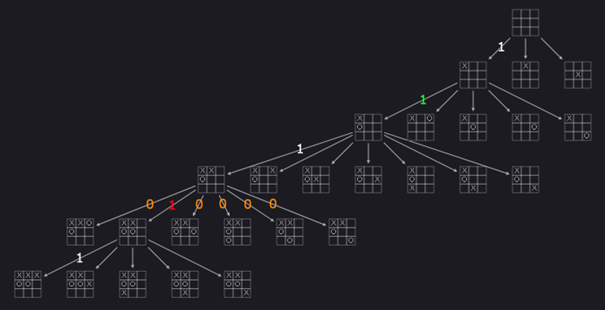
\includegraphics[width = \linewidth]{elimination1.png}
\caption{Eliminationsgewichte}
\label{elimination1}
\end{figure}

Angenommen wir haben ein Spiel zwischen einem Menschen (X) und einer EliminationsKI (O). Der menschliche Spieler ist zuerst am Zug. Die Gewichte der KI könnten wie im Bild aussehen. (Hinweis: Genau so eine Gewichtung wird im Spiel nicht vorkommen. Sie ist nur für die Veranschaulichung geeignet. Außerdem existieren für alle Kanten Gewichte. Nur die für die Belohnung relevanten Gewichte sind eingezeichnet.) 

Wird in diesem Fall die Belohnung der EliminationsKI durchgeführt, wird zuerst die rote 1 auf 0 gesetzt, da dies der letzte Zug der KI war und sie verloren hat. Denn sie hat damit dem Gegner erlaubt einen Zug zu machen, welcher den Gegner gewinnen lässt.
Daraufhin wird überprüft, ob es Spielzustände gibt, von denen aus es nur 0-Gewichte gibt. Da die rote 1 zu einer 0 geändert wurde, sind von dem Spielzustand darüber nur Züge mit Gewicht 0 möglich. Aus diesem Grund wird die grüne 1 auch auf 0 gesetzt. Denn dies war der vorherige Zug der KI, welcher es dem Gegner erlaubt hat, die KI mit einem schlauen Zug in einen Spielzustand zu bringen, aus dem für die KI nur Züge mit Gewichtung 0 folgen. 

Hinweis: Angenommen, die Rollen wären bei gleichem Spielverlauf vertauscht, die KI hätte also das Zeichen X, sie hätte angefangen zu spielen und hätte gegen den Menschen gewonnen, würden sich die Gewichte der KI genauso ändern, da sie auch von den Zügen des Gegners lernt. 


\end{document}
